\chapter{Strategic Bidding Model}
Chapter 4 explores the impact of imperfect foresight and assumes the BESS has autonomous dispatch and can discharge and charge at any given price. In reality a AEMO requires a stand-alone battery submit a separate offer (scheduled generating unit) and bid (scheduled load) into the market systems, represented by two unlinked DUIDs.
Figure \ref{fig:bidding_nem} explains the bidding process in simple terms, whereby bids to produce electricity are received by AEMO are stacked in price order for each dispatch period. Generators are then progressively scheduled into production to meet demand, starting with the lowest cost generator. In this sense, bidding alters the valuation for utility storage. The impact is ultimately minimum and maximum thresholds are set which ensure dispatch. For instance if the price is forecasts to be \$100/MWh and the generator DUID bid in all their quantity at \$300/MWh but in the next 5 minutes another generator re-bids at sets the price at \$2,000/MWh the BESS would be instructed to dispatch all the quantity even if the forecast was incorrect. The nature of bidding also has short-comings in revenue as choosing the correct bid price bands determines whether dispatch will occur. Taking the previous example, id the BESS had allocated all their quantity into their next price bands, let's say \$5000/MWh, they would effectively miss the price spike.
\begin{figure}[H]
    \centering
    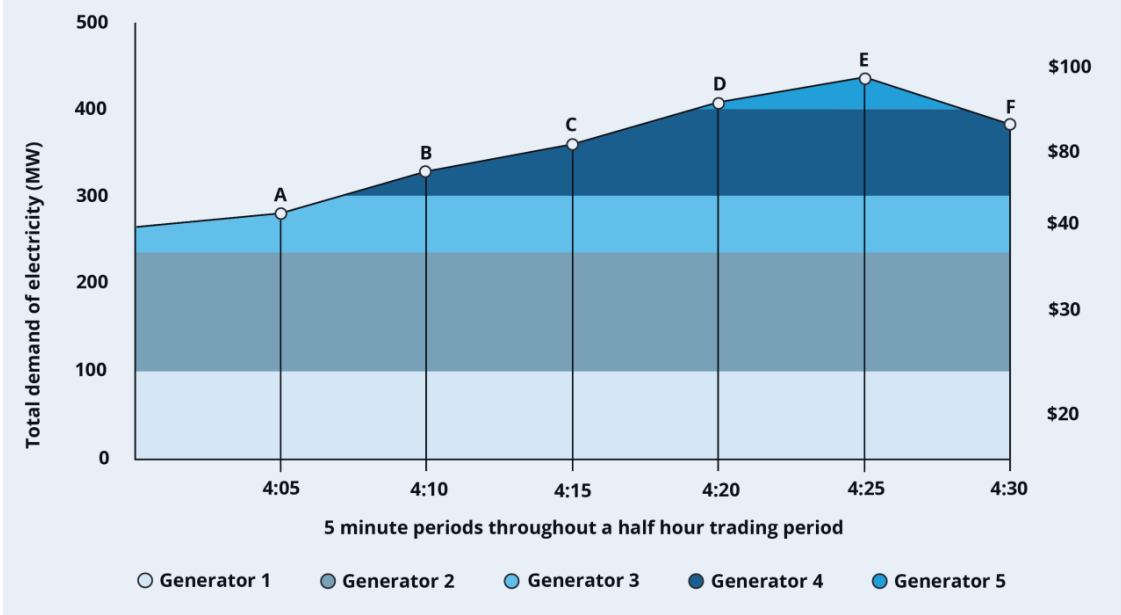
\includegraphics[width=0.7\textwidth]{Pictures/Chapter5/bidding.png}
    \caption{Scheduling generators in the NEM \parencite{AEMC_Bidding}}
    \label{fig:bidding_nem}
\end{figure}
\section{ A `crude' bidding approach}
\label{sec:crude}
This `crude' algorithm heavily relies on the work of Daniel Tam (co-author), and explores a simple bidding methodology which is to capture the price differential between 2 fixed thresholds. Conceptually this is similar to the bidding process in the NEM, however this `crude' methodology implies only once price band is set for each DUID. In practice the 10 price bid bands can be reset each day at 12:00pm, but the results below only use a static pair of upper (U) and lower (L) price thresholds.
\subsection{Methodology}
Below Algorithm \ref{alg:crude} shows the dynamic procedure to dispatch the BESS under a crude bidding methodology.
\begin{algorithm}
\setstretch{1.4}
\caption{Crude Arbitrage Algorithm}\label{alg:crude}
\begin{algorithmic}[1]
\Procedure{Dispatch}{rrp, $E_{\max}$, $P_{\max}, U , L, T, t_{\text{len}}$}
\State $t \gets 0$
\State $ E^{(0)} \gets 0$ \Comment{Initial Storage level at 0}
\While{$t < T$}
    \If{rrp$[t] \geq U $} \Comment{Discharge}
        \State $x \gets \min\left\{E^{(i)} \div \frac{t_\text{len}}{60}, P_\text{max}\right\}$
        \State  $E^{(i)} \gets E^{(i)} - x \times t_{\text{len}} \times \frac{1}{\eta_d}$
        \State $D[t] \gets x $
    \ElsIf{rrp$[t] \leq L$} \Comment{Charge}
        \State $x \gets \min\left\{(E_{\max} - E^{(i)}) \div \frac{t_\text{len}}{60}, P_\text{max}\right\}$
        \State $E^{(i)} \gets E^{(i)} + x \times t_{\text{len}} \times \eta_c$
        \State $D[t] \gets x $
    \Else \Comment{Do Nothing}
        \State $D[t] \gets 0$ 
    \EndIf
    \State $t \gets t + 1 $
\EndWhile\label{euclidendwhile}
\State \textbf{return} $D$
\EndProcedure
\end{algorithmic}
\end{algorithm}
{\renewcommand{\arraystretch}{2}}
\begin{center}
    \begin{tabular}{p{0.8cm} p{5.5cm} p{0.8cm} p{5.5cm}}
    \textbf{Constants} & & \textbf{Variables} & \\
    $P_{max}$ & Power Capacity of BESS (MW) & $x^{(i)}$ & Dispatch power at time $i$ (MW)  \\ 
    $E_{max}$ & Storage Capacity of BESS (MWh) & $E^{(i)}$ & Storage level at time $i$ (MWh) \\
    $l$ & length of time interval in minutes & & \\
    $\eta_c$ & Charge efficiency (\%) & &\\
    $\eta_d$ & Discharge efficiency (\%) & &\\
    rrp$[i]$ &  Energy price at time $i$ (\$/MWh) & &\\
    $T$ &  Total number of time intervals & &\\
    $U$ &  Upper price threshold & &\\
    $L$ &  Lower price threshold & &\\
    \end{tabular}
\end{center}
\subsection{Results}
Figure \ref{fig:crude_sample} shows a sample output of the crude bidding methodology with a 1MW BESS with 2 hours storage. The upper and lower bounds set were $U = 300$ \$/MWh and $L = 70$ \$/MWh. As this simple example highlights, the crude logic performs very well. The BESS was able to charge during the morning and capture one of the price spikes. 
\begin{figure}[H]
    \centering
    \includegraphics[width=\textwidth]{"Pictures/Chapter5/crude".pdf}
    \caption{1MW / 2MWh BESS Output Under Crude Bidding Methodology (South Australia, 19-01-2018)}
    \label{fig:crude_sample}
\end{figure}
In total the BESS made \$14,387.00 in this period, whilst the optimal perfect foresight dispatch makes \$18,197.00. Figure \ref{fig:crude_sample} raises the question; can we improve revenue if we vary the upper and lower bound thresholds. Below Figure \ref{fig:crude_thresholds} shows annual revenue in SA via varying $U$ and $L$ price thresholds from \$0 to \$300.
\begin{figure}[H]
    \centering
    \includegraphics[width=\textwidth]{"Pictures/Chapter5/crude_thresholds".pdf}
    \caption{Crude Revenue Varying Price Thresholds 1MW/2MWh BESS
South Australia, 2018}
    \label{fig:crude_thresholds}
\end{figure}
Figure \ref{fig:crude_thresholds} highlights that the ideal thresholds are charging below \$140/MWh and greater than \$180/MWh capturing approximately \$560k or 24.4\% of the \$2.292m  optimal revenue for the same scenario. Additionally it's clear that if $L>U$ then no revenue is achievable - this is logical. 
\section{Strategic Bidding Model using Linear Programming}
As explored in Section \ref{sec:crude}, the crude algorithm offers a simple operating strategy aligned with the bidding requirements in the NEM. However, the key limitation of the crude methodology is that the price bid bands are entirely static. 

\begin{tcolorbox}[colback=ocre!5!white,colframe=ocre]
``Furthermore, “buy low, sell high” is not as easy as it sounds. The energy market is incredibly complex. In our experience, a successful bidding strategy needs to be underpinned by advanced predictive analytics and co-optimisation. Failure to do so can result in the asset significantly undershooting revenue expectations. Some food for thought as the race to build big batteries begins." - \textbf{Marija Petkovic, Founder \& Managing Director of Energy Synapse}
\end{tcolorbox}
\subsection{Methodology}
Figure \ref{fig:bidding_strategy_diagram} describes the methodology undertaken to simulate a realistic bidding strategy to capture energy arbitrage revenue. As shown in Figure \ref{fig:bidding_strategy_diagram} this model combines elapsed prices, the P5 predispatch forecast and the P30 predispatch forecast. As the elapsed 5 minute prices are combined with the balance of P5 intervals within a respective trading interval, the forecast accuracy of the battery becomes progressively better as the BESS throughout the trading interval. As such, this method requires a \textit{5 minute} dispatch algorithm. Computationally this is very intensive as the model must run an LP solver on a combined forecast 105120 times a year.
\begin{figure}[H]
    \centering
    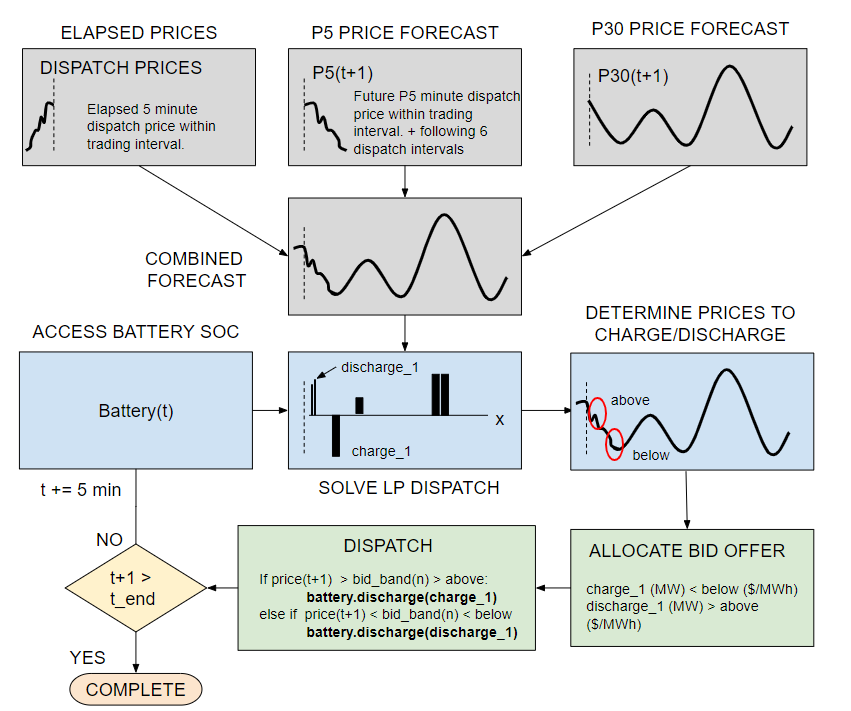
\includegraphics[width=0.7\textwidth]{Pictures/Chapter5/bidding_strategy.png}
    \caption{Energy Arbitrage Methodology using Strategic Bidding Model}
    \label{fig:bidding_strategy_diagram}
\end{figure}
Once the combined forecast is imported, the LP solver determines the first charge and discharge price/quantity pairs. For example, the first charge price may occur at \$60/MWh for a quantity of 1MW 6 intervals ahead, and the first discharge may occur at \$100/MWh for a quantity 11 intervals ahead. These price/quantity pairs are then used to inform quantity allocation into the chosen 10 price bid band. This methodology \textbf{does not} attempt to determine the optimal price bands to use. Alternatively frequently used price bands for the Hornsdale Power Reserve were extracted from AEMO MMS Table BIDDAYOFFER. Table \ref{tab:hpr_bid_bands} represent the most frequently used bid price bands by quarter for the Hornsdale Power Reserve Load and Generator DUIDs.
\begin{center}
\begin{table}[]
\centering
\begin{tabular}{|l|l|l|l|l|}
\hline
\textbf{LOAD BID BANDS}      & \textbf{Q1} & \textbf{Q2} & \textbf{Q3} & \textbf{Q4} \\ \hline
1                  & -988.6      & -988.6      & -988.6      & -985.3      \\ \hline
2                  & -500        & -500        & -500        & -500        \\ \hline
3                  & 0           & 0           & 0           & -50         \\ \hline
4                  & 30          & 30          & 30          & 25          \\ \hline
5                  & 60          & 60          & 60          & 50          \\ \hline
6                  & 90          & 90          & 90          & 90          \\ \hline
7                  & 150         & 120         & 150         & 120         \\ \hline
8                  & 300         & 150         & 300         & 150         \\ \hline
9                  & 1000        & 300         & 1000        & 300         \\ \hline
10                 & 5000        & 899         & 5000        & 899         \\ \hline
\textbf{GENERATOR BID BANDS} & \textbf{Q1} & \textbf{Q2} & \textbf{Q3} & \textbf{Q4} \\ \hline
1                  & 90          & -984.8      & -970        & -977.1      \\ \hline
2                  & 150         & 0           & 0           & 0           \\ \hline
3                  & 200         & 90          & 90          & 60          \\ \hline
4                  & 250         & 120         & 120         & 90          \\ \hline
5                  & 300         & 200         & 200         & 175         \\ \hline
6                  & 450         & 300         & 300         & 250         \\ \hline
7                  & 600         & 450         & 450         & 400         \\ \hline
8                  & 1000        & 1000        & 1000        & 1000        \\ \hline
9                  & 5000        & 5000        & 5000        & 2000        \\ \hline
10                 & 13984.16    & 13500       & 13500       & 10027       \\ \hline
\end{tabular}
\caption{Hornsdale Power Reserve - Frequently used price bid bands 2018}
\end{table}
\label{tab:hpr_bid_bands}
\end{center}
\subsubsection{Limitations}
This method has the limitation that only one quantity is assigned into a bid band. Taking the example above, if first discharge of 1MW may occur at \$100/MWh for a quantity 11 intervals ahead, and it's Q1 2018, the battery will allocate the full 1MW quantity into the 2nd bid band. Splitting the quantity across multiple bid bands isn't explored in this methodology.
\newpage
\subsection{Results}
\label{sec:strategic_bidding}
Figure \ref{fig:strategic_bidding}  highlights the result of this strategic bidding methodology for a 1MW/2MWh BESS in South Australia in 2018. As the Figure highlights this methodology of using Linear Programming on a combined forecast yields 16\% greater revenue than the `crude' algorithm presented in Section \ref{sec:crude}. \textbf{ Overall this algorithm captures 57\% of the optimal `perfect foresight' revenue. }
\begin{figure}[H]
    \centering
    \makebox[\textwidth][c]{    \includegraphics[width=\textwidth]{"Pictures/Chapter5/strategic_bidding_outcomes".pdf}}
    \caption{Caption}
    \label{fig:strategic_bidding}
\end{figure}
As mentioned in Section \ref{sec:ifn}, Infigen Energy have invested in a \$38 million BESS project, including \$10 million in state and federal funding, for a 25MW/52MWh Battery in South Australia. As shown in Figure \ref{fig:strategic_bidding}, we can conservatively estimate for energy abritrage revenue for a 2 hour storage BESS is \$100,000/MW. Hence, for the Lake Bonney BESS, a very simple calculation based on Figure \ref{fig:strategic_bidding} would suggest the LB BESS could generate \$25 million over a 10 year period \footnote{Assuming the Battery has a performance warranty of 10 years (similar to the power wall \url{https://www.tesla.com/sites/default/files/pdfs/powerwall/Powerwall_2_AC_Warranty_AUS-NZ_1-0.pdf})}. This is excluding battery performance degradation, operational costs, significant variation in price dynamics or discounting cash flows. As such, it is clear that BESS projects are still non-financial based on energy arbitrage revenue alone. Section \ref{sec:coop_method} explores additional revenue streams which battery storage can access via FCAS participation. 

